\chapter{Teoría de la Probabilidades} \label{cap:teo_prob}
	\lipsum[5] \lipsum[4]
	
	De lo visto en el capítulo \ref{cap:teo_medida} veremos \lipsum[1]
	
	\begin{figure}[h]
		\centering
		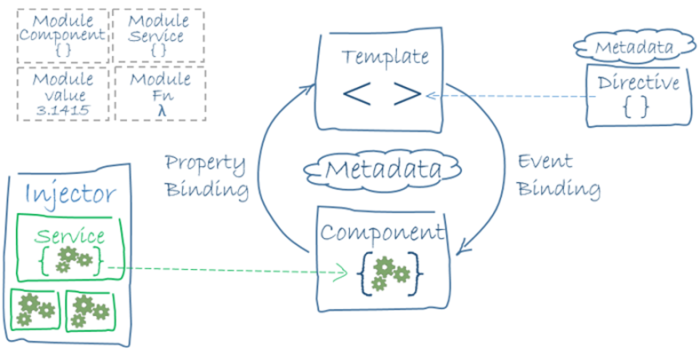
\includegraphics[scale=0.5]{imagenes/arqui_angular.png}
		\caption{Aquitectura Angular}
		\label{fig:imgen_1}
	\end{figure}